\documentclass[../../main.tex]{subfiles}
\begin{document}

\subsection*{8.12}
Un conduttore cilindrico molto lungo di raggio $a = 2\ cm$ ha nel suo interno una cavità cilindrica di raggio $b = 0.3\ cm$, essa pure molto lunga. Gli assi dei due cilindri sono paralleli e distano $d = 1\ cm$. Nel conduttore fluisce una corrente $i = 20\ A$, distribuita uniformemente.\\
Dimostrare che il campo magnetico $\vec{B}$ all'interno della cavità è costante, calcolandone modulo e direzione.\\
Calcolare inoltre l'energia magnetica e l'induttanza per unità di lunghezza del conduttore.\\
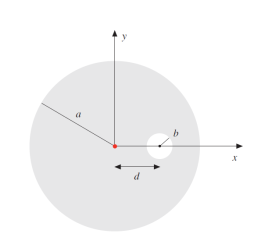
\includegraphics[scale=0.3]{e_8_12_0.png}\\
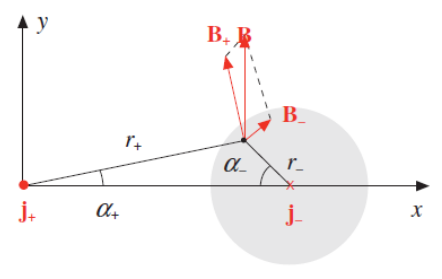
\includegraphics[scale=0.3]{e_8_12_1.png}
\subsubsection*{Formule utilizzate}
$\oint\vec{B}d\vec{s}=\mu_0i_{conc}$
\subsubsection*{Soluzione punto a}
Per risolvere questo problema, che sembra non avere semplificazione poichè non ha simmetria, in realtà possiamo considerare il foro interno come la somma di due campi opposti che si annullano fra loro.\\
A questo punto troviamo ad avere il campo di un cilindro + una carica inversa in un cilindro più piccolo interno. 
Questo si può fare per il principio di sovrapposizione.

\subsubsection*{Soluzione punto b}
\newpage

\end{document}